\documentclass[preprint2]{aastex}
\usepackage{natbib}
\usepackage{xcolor}
\usepackage{booktabs}
\bibliographystyle{apj}

\pagenumbering{gobble}

\shorttitle{Bright Point Size}
\shortauthors{Farris}

\begin{document}

\title{Determining coronal bright point size via cross-correlation using
multi-wavelength images from AIA/\textit{SDO}}
\author{Laurel Farris, R. T. James McAteer}
\affil{New Mexico State University}
\email{laurel07@nmsu.edu}

\begin{abstract}
\end{abstract}
\keywords{Sun: corona{-}Sun: bright points{-}}

\section{Introduction}\label{intro}
It is currently thought that after magnetic flux tubes rise from the tachocline
of the sun (between the convection and radiative zones) to the photosphere, they
are moved across the photosphere by the process of advection to the junctions
between supergranules (source?). There they are observed as bright points (BPs).
Though they only cover about 1.6 \% of the
photosphere (\cite{Srivastava}), BPs (together with sunspots)
contribute over 90\% of the total magnetic flux (\cite{Howard}).
Over the course of the solar cycle, they can contribute significantly to the
global intensity variation of the sun, particularly in the ultraviolet
regime (\cite{Riethmuller}).

These BPs can be seen in the upper layers of the solar atmosphere in the form
of coronal BPs. The cross-sectional area of these BPs is known to increase with
height above the photosphere as the density decreases and temperature increases
(source?).

Several techniques for determining the size of coronal BPs have been investigated
in the literature.
\cite{Alipour} developed an algorithm to locate BPs in the corona, using size determined
by intensity as part of the criteria for distinguishing BPs from other features,
such as top-down views of coronal loops or nanoflares.

The goal for the project discussed in this Letter was to determine size in another
way, using the cross-correlation between the pixels in and around the visible
area occupied by the BP. The data is described in \S{} \ref{data},
the analysis is discussed in \S{} \ref{analysis},
and conclusions are in \S{} \ref{conclusion}.


\section{Data}\label{data}
This analysis was carried out using multi-wavelength data from AIA/\textit{SDO}
spanning one hour on June 1, 2012 from 13:00:00 to 13:59:59, at a cadence of 12
seconds.
Each EUV passband corresponds to emission
from different transitions of ion species in the corona, each of which takes
place at different temperatures, and hence different heights, above the
photosphere.
The relevant values for each passband are given in table \ref{temps}.
\begin{table}[h]
\centering
    \begin{tabular}{l l l}
        \hline\hline
        Wavel. [\AA{}] & log(T) [K] & Ion(s) \\
        \hline
        94 & 6.8 & Fe {\small XVIII} \\
        131 & 5.6, 7.0 & Fe {\small VIII, XXI} \\
        171 & 5.8 & Fe {\small IX} \\
        193 & 6.2, 7.3 & Fe {\small XII, XXIV} \\
        211 & 6.3 & Fe {\small XIV} \\
        304 & 4.7 & He {\small II} \\
        335 & 6.4 & Fe {\small XVI} \\
    \end{tabular}
\caption{Characteristic temperatures corresponding to the wavelengths observed
    in emission in the solar corona (from \cite{Lemen}).}
\label{temps}
\end{table}

A grayscale image of the full disk at the beginning of the time series for each
bandpass is shown in figure \ref{full}.
A single BP from a coronal hole located in the full disk was selected for analysis.
Grayscale images showing this BP in each passband are shown in figure \ref{bp_images}.

\begin{figure*}[htb!]
    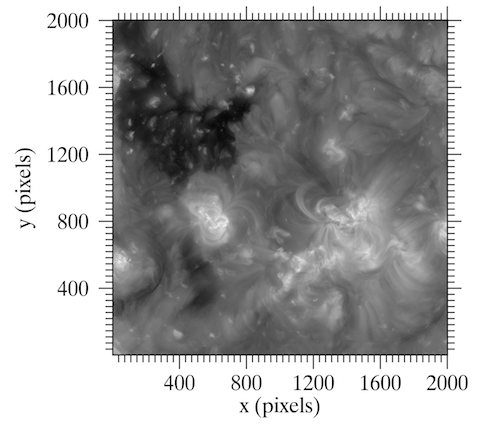
\includegraphics[width=\textwidth]{Figures/full.png}
    \caption{Full disk showing the relative intensity at the start of the time
        series for each AIA bandpass used in this study.}
    \label{full}
\end{figure*}

\begin{figure*}[htb!]
    \includegraphics[width=\textwidth]{Figures/images.png}
    \caption{Images of the BP in six different AIA wavelengths. The pixel coordinates
        are given relative to the full disk shown in figure \ref{full}.
        The location of the BP appears to shift from one bandpass to next, which
        may indicate a structure that is not completely straight, or a possible shift
        in the data itself.}
    \label{bp_images}
\end{figure*}

\section{Analysis}\label{analysis}
The intensity of each BP as a function of radius gives a visual estimate
of the size of the BP. For comparison, the intensity of the first image in each
passband is plotted as a function of radial distance from the center pixel in figures
\ref{intensity_1} and \ref{intensity_2}.

For this project, the size was estimated by running a cross-correlation between
a pixel roughly in the center of the BP and the remaining pixels over the
100 $\times$ 100 pixel$^{2}$ area through the full time series.
The central pixel was arbitrarily determined by locating the brightest pixel in the center
of the BP from the first image in the time series. The cross-correlation analysis
helped to determine what parts of the feature were moving together as a single
physical structure.

\section{Results}\label{results}

\subsection{Cross-correlation as a size indicator}
Images illustrating the highest cross-correlation value of each pixel and the
timelag corresponding to that correlation value are shown in figures \ref{cc_all}
and \ref{tt_all}. The correlation was cut off at 0.5 and rescaled to obtain a
better illustration of the structure of the BP. These images are shown in
figures \ref{cc} and \ref{tt}.

As \cite{Alipour} noted, the BP structure is most evident for the
131\AA{}, 193\AA{}, and 211\AA{} images.

\subsection{Variation in BP size with temperature}
Even though the temperature of the corona increases with height from the transition
region to wherever the corona actually ends (need source here), there is not necessarily
a direct correlation between temperature and absolute height above the photosphere
due to the variety of structures
and overall inhomogeneity that exists in the solar atmosphere (\textcolor{red}{source}).
However, the \emph{relative} height between each bandpass for a given structure is
possible to determine, and is relevant to this study.

\subsection{Extra emission in 211\AA{}}
The 211\AA{} data is particularly notable as it shows strong correlation values
at two points to the right of where the BP appears visually in figure \ref{full}.
This could be the result of a jet of light emitted from the main structure, or a
possible indicator of the main structure splitting into several tubes at the
height where the 211 \AA{} emission is strongest.
A movie showing all images from this wavelength (\cite{ssw}) revealed a flash
of emission around the 45th image,
which matches the timelag at which the high correlation values occurred as shown
in figure \ref{closeup}.

\begin{figure*}[htb!]
    \includegraphics[width=\textwidth]{Figures/cc_all.png}
    \caption{Images showing the highest cross-correlation value for each pixel. }
    \label{cc_all}
\end{figure*}

\begin{figure*}[htb!]
    \includegraphics[width=\textwidth]{Figures/tt_all.png}
    \caption{Images showing the timelag corresponding to the correlation values
        illustrated in figure \ref{cc_all}.}
    \label{tt_all}
\end{figure*}

\begin{figure*}[htb!]
    \includegraphics[width=\textwidth]{Figures/cc_images.png}
    \caption{Cross-correlation images scaled to show only values higher than 0.5.}
    \label{cc}
\end{figure*}

\begin{figure*}[htb!]
    \includegraphics[width=\textwidth]{Figures/tt_images.png}
    \caption{Timelag corresponding to the cross-correlation values higher than 0.5.}
    \label{tt}
\end{figure*}

\begin{figure*}[htb!]
    \includegraphics[width=\textwidth]{Figures/im_211.png}
    \caption{Images from the 211 \AA{} bandpass only, around the times when the
        two jets of light appeared in the upper right region of the main body of the BP. }
    \label{tt}
\end{figure*}

\begin{figure*}[htb!]
    \includegraphics[width=\textwidth]{Figures/closeup_211.png}
    \caption{Timelag at 211 \AA{} ``zoomed in'' around the two jets of light.}
    \label{closeup}
\end{figure*}

\begin{figure*}[htb!]
    \includegraphics[width=\textwidth]{Figures/intensity_1.png}
    \caption{Intensity of each pixel is plotted as a function of radius for each
        passband. I have no idea what's going on with the 94\AA{} data.}
    \label{intensity_1}
\end{figure*}

\begin{figure*}[htb!]
    \includegraphics[width=\textwidth]{Figures/intensity_2.png}
    \caption{Same as figure \ref{intensity_1}, but with half the radius range
        cut off to better view the values around the main BP.}
    \label{intensity_2}
\end{figure*}

\begin{figure*}[htb!]
    \includegraphics[width=\textwidth]{Figures/cc_tt_plot.png}
    \caption{The highest cross-correlation value of each pixel is plotted as a function
        of its distance from the center pixel. The color indicates the timelag
        corresponding to the maximum cross-correlation for that pixel.}
    \label{tt_all_plot}
\end{figure*}

\begin{figure*}[htb!]
    \includegraphics[width=\textwidth]{Figures/cc_tt_plot_scaled.png}
    \caption{Same as figure \ref{tt_all_plot}, but with two thirds of the timelag cut out
        at both ends.}
    \label{tt_plot}
\end{figure*}


\section{Conclusion}\label{conclusion}

\bibliography{reffile}
\end{document}
